\documentclass[11pt]{article}
\usepackage{amssymb,amsmath,amsthm,graphicx}
\usepackage{fancyhdr}

\def\shownotes{1}   % set 1 for version with author notes
                    % set 0 for no notes



%uncomment to get hyperlinks
%\usepackage{hyperref}

%%%%%%%%%%%%%%%%%%%%%%%%%%%%%%%%%%%%%%%%%%%%%%%%%%%%%%%%%%%%%%
%Some macros (you can ignore everything until "end of macros")

\topmargin 0pt \advance \topmargin by -\headheight \advance
\topmargin by -\headsep

\textheight 8.9in

\oddsidemargin 0pt \evensidemargin \oddsidemargin \marginparwidth
0.5in

\textwidth 6.5in

%%%%%%

\providecommand{\vs}{vs. }
\providecommand{\ie}{\emph{i.e.,} }
\providecommand{\eg}{\emph{e.g.,} }
\providecommand{\cf}{\emph{cf.,} }
\providecommand{\etc}{\emph{etc.} }

\newcommand{\getsr}{\gets_{\mbox{\tiny R}}}
\newcommand{\bits}{\{0,1\}}
\newcommand{\bit}{\{0,1\}}
\newcommand{\Ex}{\mathbb{E}}
\newcommand{\eqdef}{\stackrel{def}{=}}
\newcommand{\To}{\rightarrow}
\newcommand{\e}{\epsilon}
\newcommand{\R}{\mathbb{R}}
\newcommand{\N}{\mathbb{N}}
\newcommand{\Gen}{\mathsf{Gen}}
\newcommand{\Enc}{\mathsf{Enc}}
\newcommand{\Dec}{\mathsf{Dec}}
\newcommand{\Sign}{\mathsf{Sign}}
\newcommand{\Ver}{\mathsf{Ver}}

\providecommand{\mypara}[1]{\smallskip\noindent\emph{#1} }
\providecommand{\myparab}[1]{\smallskip\noindent\textbf{#1} }
\providecommand{\myparasc}[1]{\smallskip\noindent\textsc{#1} }
\providecommand{\para}{\smallskip\noindent}


\newtheorem{theorem}{Theorem}
\theoremstyle{definition}
\newtheorem{ex}{Exercise}
\newtheorem{definition}{Definition}

%%%%%%%  Author Notes %%%%%%%d
%
\ifnum\shownotes=1
\newcommand{\authnote}[2]{{ $\ll$\textsf{\footnotesize #1 notes: #2}$\gg$}}
\else
\newcommand{\authnote}[2]{}
\fi
\newcommand{\Snote}[1]{{\authnote{Solution}{#1}}}
\newcommand{\Inote}[1]{{\authnote{Solution}{#1}}}
\newcommand{\Ichanged}[1]{{\authnote{Changed}{#1}}}
%%%%%%%%%%%%%%%%%%%%%%%%%%%%%%%%%

\newcommand{\VAR}{\mathrm{VAR}}



% end of macros
%%%%%%%%%%%%%%%%%%%%%%%%%%%%%%%%%%%%%%%%%%%%%%%%%%%%%%%%%%%%%%


% page counting, header/footer
\usepackage{fancyhdr}
\pagestyle{fancy}
\lhead{\footnotesize \parbox{11cm}{CS455, Boston University, Fall 2015} }
\rhead{Erik Brakke}
\renewcommand{\headheight}{24pt}

\begin{document}

\title{PA 1}
\author{Erik Brakke}
\maketitle

\thispagestyle{fancy}
 
 
\section*{Compilation Instructions  Design}
\begin{enumerate}
\item[Part 1]
To run the client, navigate to the containing folder, and then run "python p1client.py HOST PORT"\\
This will connect the client to the host at the specified port, and will send the message "Default Message"\\
\newline
Design decisions:  This client is very simple.  It makes sure that a host and a port number are specified before trying to start a connection.  The port must be a valid digit in order for the connection to take place.  I did not include any default settings for the client as I found that to be unnecessary.  The client then connects, send a predefined message, and the receives a message of up to 1024 bytes.  I settled on 1024 bytes because there is not message format, so the line has to be drawn somewhere for the client to stop receiving bytes from the server.  
\newline
To run the server, navigate to the containing folder and run "python p1server.py PORT"\\
This will start the server on the specified port and it will begin to accept connections.  \\
\newline
Design decisions: The server will accept a port number as an argument to start, though I decided to include a default value for the port as well.  The server then initializes a socket and uses the socket functions to obtain the hostname.  I chose not to listen on all interfaces, and this provides unncessesary exposure for the server.  The server will only listen to 1 connection at a time (no buffer for connections).  I chose to do this because this is not a multithreaded server.  I do not want a client to wait on the server to finish the previous process, I just want them to be able to connect when the server is able to process their request.  A possible extention of the server would be to make it a multithreaded server, and then I could accept and process many connections are the same time.  The server will only accept messages of 1024 bytes in length.  Again this is because there is not message format, so the distinction has to be drawn somewhere.  No errors are sent to the client.  A possible extention would be to include error communication with the client.
\item[Part 2]
To run the client, navigate to the containing folder and run "python p2client.py HOST PORT MEASUREMENT\_TYPE NUM\_PROBES MESSAGE\_SIZE [SERVER\_DELAY]".  In the case of "rtt", the message size must be a valid integer $>$ 0.  In the case of "tput", the message size must be a valid integer with "K" appended to it to denote kilobytes.  Server Delay is optional and will default to 0 if omitted\\
\newline
Design decisions: The client will validate these inputs before starting the protocol with the server.  This is to ensure that as long as the server behaves correctly, then the client should have no problems talking to it.  I chose to make server delay only integer values in this case.  I felt that this accomplished the idea of server delay well enough, though if I were to turn this into a more fine tuned network analysis tool, I would allow for server delay to be specified in milliseconds.  In the setup phase, the client will accept two different ready responses.  This is because the assignment states that "200 OK: Ready\textbackslash n" is what the server should return, though it was observed that the servers actually returned "200 OK:Ready\textbackslash n".  The client will then go through the measurement phase and keep track of the amount of time it takes to receive the message.  It will then either keep the times (RTT) or it will convert them to throughput (kbps). \\
\newline
To run the server, navigate to the containing folder and run "python p2server.py PORT".  This will start the server on the specified port.\\
\newline
Design decisions: The server will only listen on the interface of the host returned by the socket function gethostname and gethostbyname.  This is so it only listenes on the interface visible to the outside.  An extension could be to allow the user to specify the host name as well.  The server only listens for 1 connection at a time.  Again, like part 1, if this were a multithreaded server, it would make sense to accept more connections, but for now listening for 1 connections at a time suffices.  There is no socket timeout on the server.  If the client sends a message without a newline, the server will become stuck in an infinite loop trying to receieve the clients message.  A possible extension would be to set socket timeouts, but again I felt it was not necessary for this assignment.

\end{enumerate}

\section{Plots}
In this section I will discuss the results of testing the RTT and throughput on multiple servers.  NOTE: I take 1K = 1000 bytes, not 1024.  Also when taking measurements with server delay, I only took 10 measurements so the experiment would not take a very long time

\subsection*{RTT on csa server}
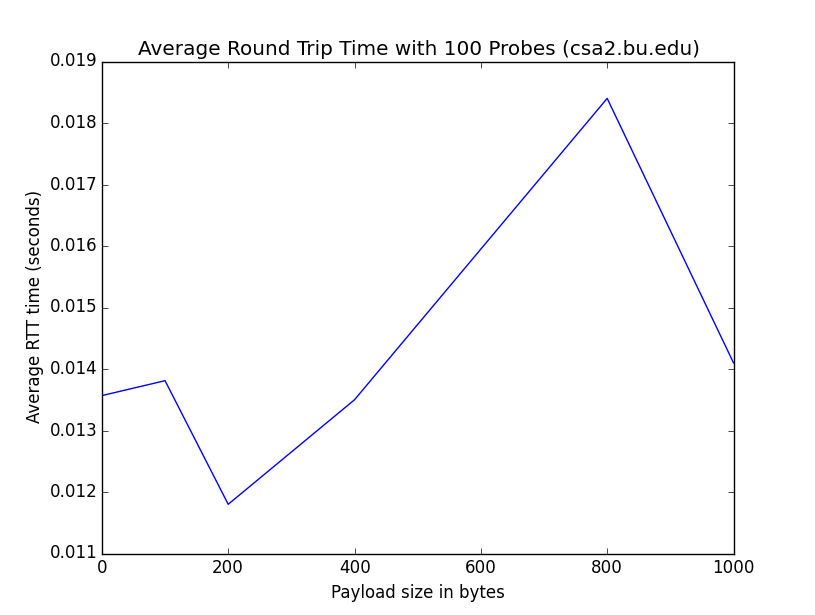
\includegraphics[scale=0.4]{rtt_csa}
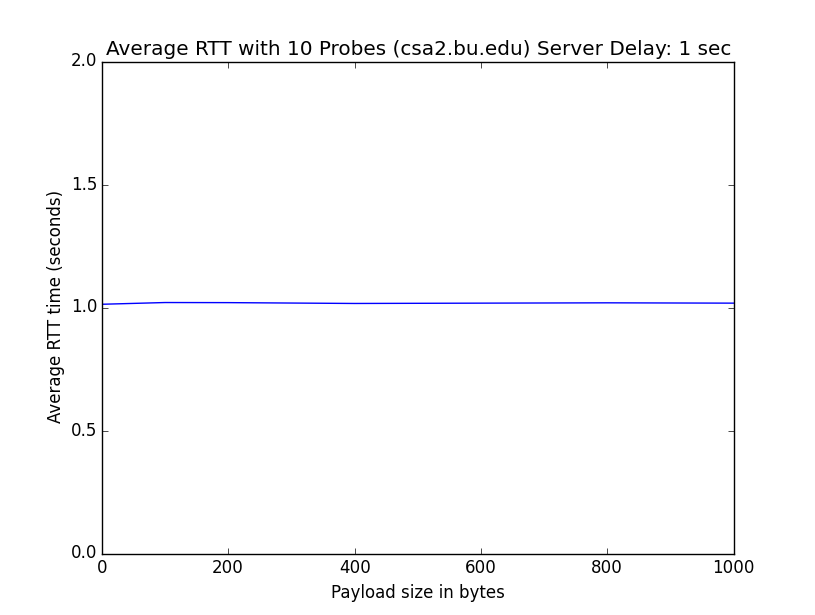
\includegraphics[scale=0.4]{rtt_csa_sd1}

From this we can see that without any server delay, the range of the RTT between payload sizes is only about 10ms.  There does not appear to be any trend that it follows.  Once a 1 second delay is added to the server, we can see that the rtt is pretty much a straight line.  This shows that when looking at RTT, the server delay is what contributes most to the message being sent and received.  The difference between sending 1 byte and 1000 bytes is very small.

\subsection*{TPUT on csa server}
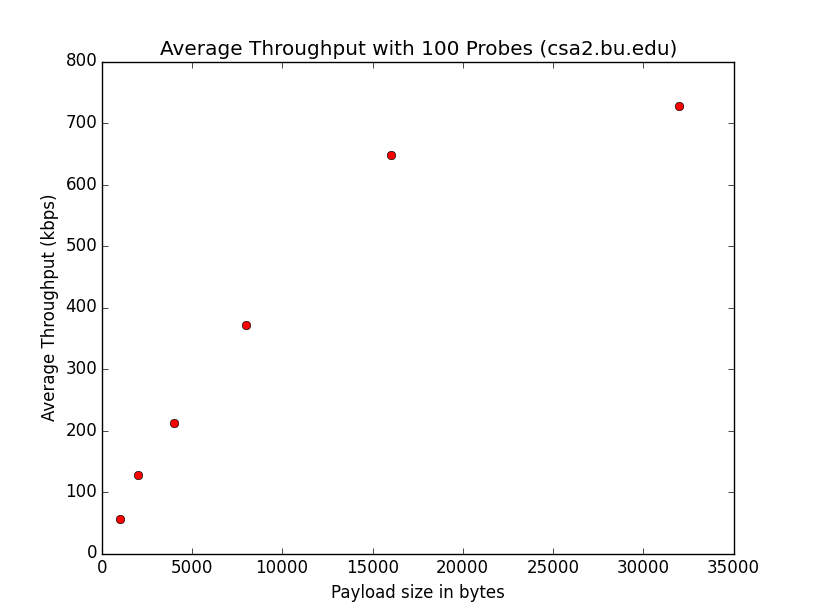
\includegraphics[scale=0.4]{tput_csa}
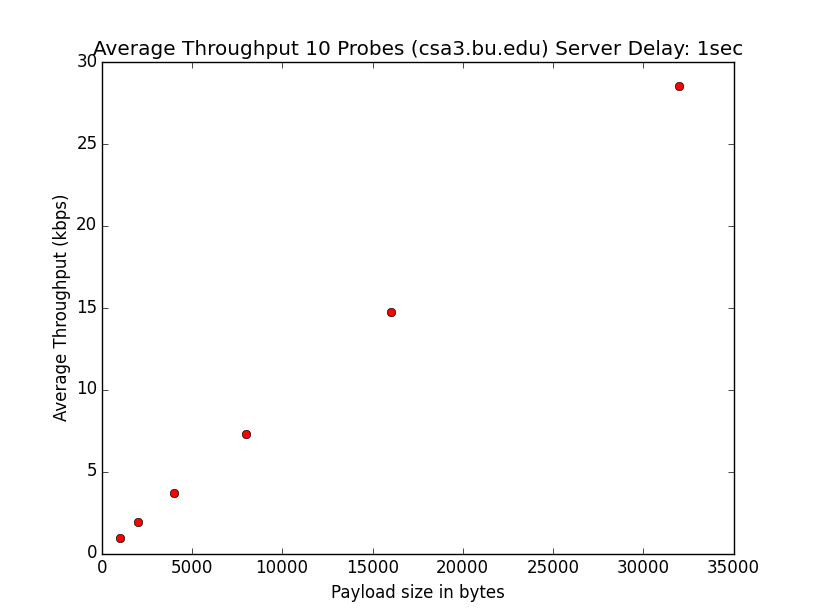
\includegraphics[scale=0.4]{tput_csa_sd1}

We can see that tput with no server delay quickly approaches a limit of about 750 kbps as the message sizes increase.  This is because as the message sizes get larger, we will hit the out maximum bandwidth that we can send to the server.  In other words, as the message gets bigger, we start to be affected by bottlenecking in the network.  However, when there is server delay, we can see that the throughput follows a more linear model.  With a 1 second delay, we see that the throughput is roughly the size of the message we are sending.  This shows us that with a 1 second delay, it is still the server delay that is the dominating factor in calculating the throughput, no the message size.  Even if we were capable of sending data at 1Mbps, if the server took 1 second to process our data, we would only get a rate of about 30 kbps when sending 32K of data.

\subsection*{TPUT and RTT on utah.geniracks.net}
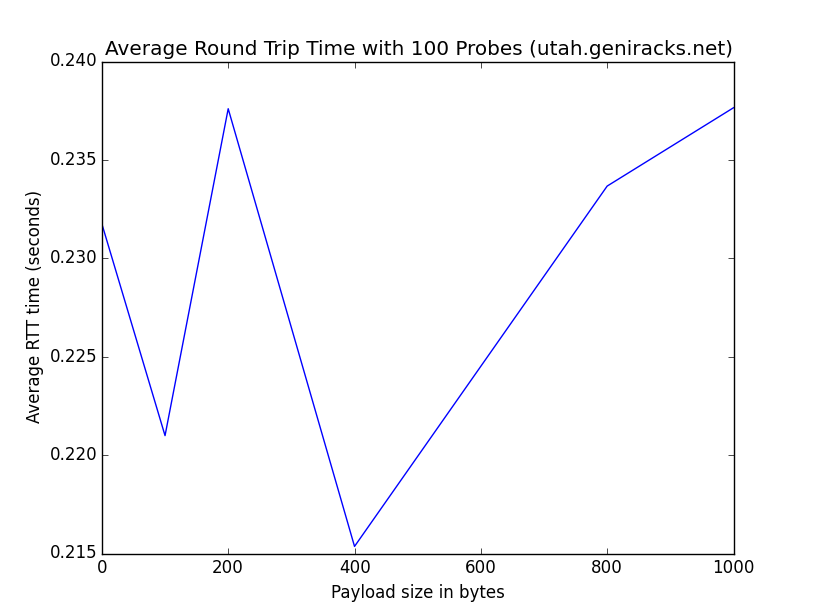
\includegraphics[scale=0.4]{rtt_utah}
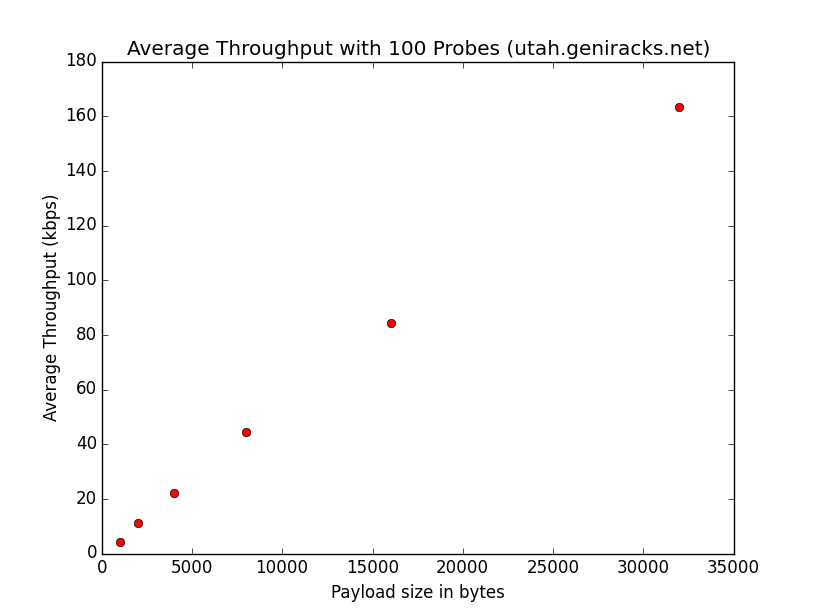
\includegraphics[scale=0.4]{tput_utah}

We can see here that the RTT to utah is on average much greater, but there is still no trend that it follows.  The range is about 20ms, but the biggest takeaway is that because utah is farther away, it takes any size packet much longer to travel there and back.  The TPUT to utah follows a more linear model than did sending backets to csa2.  This is most likely because utah is farther away, so there is more propagation delay.  The message has to travel through more routers along the way which will give us a lower TPUT time.  So even if Utah had a line that could accept messages at 1mbps and I had a line that could send and receieve at 1mbps, the throughput I get to Utah could be much less than 1mbps due to the delay of the routers on the path to utah.  Also, if the server has a lot of load, then it will not necessarily be able to process my request right away, which would lead to even less throughput.  


\end{document} 